\documentclass[a4paper, UTF8]{ctexart}

\usepackage{amsmath}
\usepackage{amssymb}
\usepackage{graphicx}
\usepackage{float}
\usepackage[hidelinks]{hyperref}
\usepackage{listings}
\newtheorem{proposition}{命题}
\DeclareMathOperator{\sgn}{\mathrm{sgn}}
\DeclareMathOperator{\trunc}{\mathrm{trunc}}
\lstset{
    basicstyle=\small\tt,
    numbers=left
}

\title{将一浮点数转换为两根式之和的最简算法}
\author{郑}

\begin{document}
\maketitle

\section{引言}
一些数值计算器在计算分数以及根式时会返回形如$\dfrac{\pi}{3}$或$\dfrac{2\sqrt{2}}{3}$这样的数学表达式,而非浮点数,同样也能显示$1+\sqrt{2}$以及$\dfrac{\sqrt{2}+\sqrt{3}}{2}$。前面两个可以通过简单的运算在一瞬间得出。但是后面两个涉及到加法运算,如果我们想分别求出$\dfrac{\sqrt{a}+\sqrt{b}}{c}$中$a,b,c$的值,最直接的方法就是使用三重for循环。但是这样子效率并不高,如何减少循环的使用并提高效率?这就是我写这篇文章的目的:介绍一种可以将一浮点数转换为两根式之和的算法。

\section{理论}
我们先从不带分母的形式开始。为了减少重复度,先定义一函数\[S(x,y)=\sgn(x)\sqrt{|x|}+\sgn(y)\sqrt{|y|} \quad x,y\in\mathbb{Z}\]若仅知浮点数$n=S(a,b)$,则可以使用一些数学技巧并仅仅使用一个while循环来求出$a$和$b$,而不是使用双重for循环。简而言之,我们是要找出$S^{-1}(x)$。

首先,使用既定的公式计算$S^{-1}(x)$是不可能的,浮点数已经损失了太多的信息。使用穷举法便成为了唯一的方法,不过使用何种方法以及设定哪个初始值是一个值得讨论的问题。前者我已经在引言处说明,接下来要讨论的是后者,首先请先看如下真命题
\begin{proposition}
    有两数之和$a+b$,且$c=\dfrac{a+b}{2}$,那么$|c-a|=|c-b|$。
\end{proposition}
根据该命题,有$n=S(a,b)$,我们可以从$\dfrac{n}{2}$处往$+\infty$或$-\infty$方向搜索,只要确定了$a$就可以有唯一的$b$,再进行一次条件判断就可以确定它们是否为所求。

当然,以$\dfrac{n}{2}$作为起始值不太妥当,我们要求的是两个整数,以截尾取整后的$\left(\dfrac{n}{2}\right)^2$作为起始值更合适。

不过,考虑$\left(\dfrac{\sqrt{100}+\sqrt{101}}{2}\right)^2\approx100.499$,截尾取整后为100,这样的设计亦有疏漏。但是,有如下极限\[\lim_{x\to+\infty} \left(\frac{\sqrt{x}+\sqrt{x+1}}{2}\right)^2-x=\frac{1}{2}\]这说明函数$f(x)=\left(\dfrac{\sqrt{x}+\sqrt{x+1}}{2}\right)^2$可近似成$x+\dfrac{1}{2}$,而且当$x>5.76$时误差小于$1\%$;$x>62.001$时误差小于$0.1\%$。

这样,即使根号内两数再接近我们也能求出它们。

以上,我们可以确定起始值
\[
    start(n)=
    \begin{cases}
        \trunc(\frac{n}{2})^2+\frac{1}{2} & \text{if }n>0 \\
        -\trunc(\frac{n}{2})^2-\frac{1}{2} & \text{if }n<0
    \end{cases}
\]

以下为了书写方便,将$\sqrt{n}$定义为$\sgn(n)|n|^{1/2}$。

已知$n=S(a,b)$,在确定了起始值$start$之后,令$step=0.5$,找到一个端点\[\alpha=start-step\]然后可计算另一端点\[\beta=\frac{n}{2}-|\sqrt{a}-\frac{n}{2}|\]由于$\beta$必须为整数,故还需做如下处理\[\beta=\sqrt{\sgn(\beta)\mathrm{round}(\beta^2)}\]其中round表示舍入到最接近的整数。

如果$\sqrt{\alpha}+\sqrt{\beta}=n$的话,那么$\alpha$和$\beta$就是要求的$a$和$b$。不然的话使$step\pm1$,向正无穷或负无穷方向继续寻找。

\section{实现}
这里给出的示例使用的是Python标准库,也可以使用mpmath等库来获得更高的精度。

\begin{lstlisting}[language=python, name=example1]
import math

def num2sqrts(n, max_num=1000):
	if n >= 0:
        mid = math.floor((n / 2) ** 2) + 0.5
    elif n < 0:
        mid = math.ceil(-(n / 2) ** 2) - 0.5
    fsqrt = lambda n: math.copysign(math.sqrt(math.fabs(n)), n)
    actual_mid = n / 2
    t = 0.5
    while True:
        a = fsqrt(mid + t)
        d = math.fabs(a - actual_mid)
        b = actual_mid - d
        b = fsqrt(math.copysign(round(b ** 2), b))
\end{lstlisting}
理论上,这个算法可以一直运行下去,直到找到合适的值。但是考虑到实际情况,我还是设置了停止条件。
\begin{lstlisting}[language=python, name=example1]
        if abs(a ** 2) > max_num or abs(b ** 2) > max_num:
            return
        if math.isclose(a + b, n):
            return int(round(math.copysign(a ** 2, a))), \
                int(round(math.copysign(b ** 2, b)))
        t += 1
\end{lstlisting}
最后,函数num2sqrts返回的是长度为2的元组,若返回值为\verb|None|则说明没有找到解析解。

\begin{figure}[htb]
	\centering
	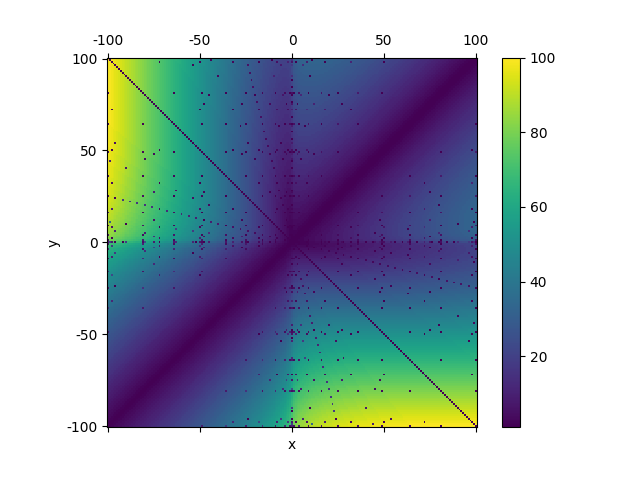
\includegraphics[width=0.8\linewidth]{perform1.pdf}
	\caption{算法的表现}
	\label{fig:perform1}
\end{figure}

为了说明这个算法的表现,我取$-100\leq x\leq100$且$-100\leq y\leq100$,计算求出$S(x,y)$中的$x$和$y$需要几次循环,并以不同的颜色标识,便绘制了图\ref{fig:perform1}。可见,当$x$和$y$的差值越大时,就需要更长的时间。

不过,当我们执行如下(或类似)语句时
\begin{lstlisting}[language=python]
num2sqrts(2 * math.sqrt(123))
\end{lstlisting}
返回的是\verb|(492, 0)|,循环执行了438次,但是$2\sqrt{123}$这个值可以通过更简单的方法算出。故我将一、三象限对角线上的值全部赋为1。

在最后,我将阐述如果增加了一个分母应该如何处理。再寻找一个新的算法的话效率就太低了,我们完全可以穷举分母。
\begin{lstlisting}[language=python, name=example2]
def num2sqrts2(value):
    for n in range(1, 100):
        if (ret := num2sqrts(value * n)) is not None:
            return *ret, n
\end{lstlisting}
穷举的范围是可以随意扩大(在这里是1--99),经过测试,所花费的时间也会呈线性的增加\footnote{数据来自\url{https://jason-bowen-zheng.github.io/num2str/perform2.json}。}。

\section{结语}
就这样好了,很简单吧!恕我就这样简简单单的结尾,不过也没什么好写的了。总之我认为这是一个非常高效的算法。

最后说一句,所有的源代码以及本文件都可以在\url{https://github.com/jason-bowen-zheng/num2str}中找到。

\end{document}
